\documentclass[11pt,a4paper]{article}

\usepackage[utf8]{inputenc}
\usepackage[T1]{fontenc}
\usepackage{lmodern}
\usepackage{geometry}
\usepackage{graphicx}
\usepackage{booktabs}
\usepackage{multirow}
\usepackage{amsmath}
\usepackage{amssymb}
\usepackage{array}
\usepackage{hyperref}
\usepackage{xcolor}
\usepackage{enumitem}
\usepackage{caption}
\usepackage{subcaption}

\geometry{margin=1in}
\hypersetup{
    colorlinks=true,
    linkcolor=blue,
    citecolor=blue,
    urlcolor=blue
}

\title{A Data-Centric Study of Fast Simulation and Low-Frequency Reconstruction for Pulmonary Electrical Impedance Tomography}
\author{Anonymous Authors}
\date{}

\begin{document}
\maketitle

\begin{abstract}
Electrical impedance tomography (EIT) reconstruction for pulmonary monitoring is a highly ill-posed inverse problem whose practical performance depends not only on the network architecture but also on simulation throughput, data complexity, and representation bias. In this work, we present a data-centric study of pulmonary EIT reconstruction built on an optimized KTC2023 codebase. We first accelerate simulation and evaluation through reduced-right-hand-side forward solving and Torch/CUDA-based fast scoring. We then compare several representation families, including pixel-wise direct prediction, continuous latent autoencoding, discrete dictionary-constrained latent modeling, and fixed low-frequency basis prediction. On the KTC benchmark, the proposed DCT ensemble reaches a total official score of 14.0553, slightly exceeding the FCUNet baseline of 14.0485. For pulmonary synthetic data, FCUNet remains the stronger reconstruction baseline with a mean score of 0.7819, while the proposed DCT model reaches 0.7272 but uses 10.6$\times$ fewer parameters and is 13.5$\times$ faster for single-sample inference and 58.3$\times$ faster in batched inference. We further show that pulmonary synthetic conductivity data are strongly atlas-dominated: a train-mean atlas already achieves a relative-$L_2$ error of 0.2553 on the 2048-sample test split, while an oracle atlas-residual DCT approximation with only $K=20$ coefficients reduces this to 0.1593. This indicates that pulmonary EIT difficulty is governed more by recovering local deviations around stable anatomy than by representing the conductivity image itself. The resulting study provides a reproducible basis for data-centric pulmonary EIT research and efficient deployable reconstruction.
\end{abstract}

\noindent\textbf{Keywords:} electrical impedance tomography, pulmonary imaging, low-frequency prior, DCT, representation learning

\section{Introduction}
Electrical impedance tomography reconstructs an internal conductivity distribution from boundary current-voltage measurements. The inverse problem is nonlinear, severely ill-posed, and highly sensitive to modeling errors and noise \cite{cheney1999eit}. These properties are especially pronounced in pulmonary EIT, where clinically meaningful structures are dominated by smooth, low-frequency variations rather than arbitrary high-frequency detail \cite{frerichs2017consensus}. This makes pulmonary EIT an especially suitable setting for testing whether explicit low-frequency priors can replace part of the burden otherwise carried by large image-space decoders.

Recent neural reconstruction methods for EIT can be roughly grouped into direct measurement-to-image mapping, latent-space inversion, and diffusion or iterative refinement. However, not all representation choices are equally suitable for pulmonary conductivity images. A representation that is too local or too discrete at the pixel level may generate fragmented structures, while a representation that is too compressed or too high-entropy may be difficult to infer from boundary measurements.

This paper summarizes a complete experimental study conducted on the KTC2023 codebase and its pulmonary extension. The study starts from engineering optimization, then compares multiple representation families, and finally reframes the pulmonary problem from a data-centric viewpoint. The resulting picture is nuanced: the DCT route is strongest on the benchmark phantom task and highly efficient on pulmonary synthetic data, while FCUNet remains the higher-accuracy pulmonary baseline at the current training scale. More importantly, pulmonary synthetic reconstruction is shown to be dominated by local deviations around a stable atlas, which changes how representation quality should be interpreted.

The main contributions are as follows:
\begin{enumerate}[leftmargin=1.5em]
    \item We optimize EIT simulation and evaluation for large-scale experimentation, including exact reduced-right-hand-side forward acceleration and Torch/CUDA-based fast scoring.
    \item We show empirically that pixel-wise discrete generation is mismatched to low-frequency conductivity structure and that latent autoencoders do not by themselves solve the measurement-to-image bottleneck.
    \item We propose and validate a fixed-basis DCT predictor that achieves the best current benchmark score in the repository and provides a strong efficiency advantage.
    \item We build and analyze pulmonary synthetic datasets with controllable anatomical and local-variation complexity, showing how atlas dominance changes with the generator settings.
    \item We extend the study to pulmonary synthetic data and show that the benchmark-optimal representation is not automatically pulmonary-optimal, and that pulmonary difficulty is governed by recovering local deviations around stable anatomy.
\end{enumerate}

\section{Related Work}
\subsection{Neural EIT Reconstruction}
Neural EIT methods typically fall into three broad categories: direct reconstruction networks, latent-variable models, and iterative generative refinement. Direct methods are attractive because of their speed and simplicity, but they rely heavily on architectural inductive bias. Latent-variable methods restrict the image space through an autoencoder and then learn a measurement-to-latent inverse map. Iterative and diffusion-based methods can improve fidelity but are generally more computationally demanding.

\subsection{Low-Frequency Priors for Conductivity Imaging}
Pulmonary conductivity distributions are dominated by anatomical regions with strong global structure and relatively smooth variation. This suggests that low-frequency or shape-constrained representations may be more appropriate than locally independent pixel-level prediction. The present work is motivated by this structural mismatch and evaluates several representation families from this viewpoint.

\subsection{Vector Quantization and Structured Latent Spaces}
Vector-quantized autoencoders constrain the image manifold through a finite codebook and can potentially suppress unrealistic outputs \cite{oord2017vqvae}. However, whether such discrete latent spaces are also easy to infer from EIT measurements remains an open question. Our experiments show that decoder-side regularity alone does not solve the inverse-map difficulty.

\section{Engineering Foundation}
\subsection{Accelerated Data Generation}
Large-scale controlled experiments require efficient simulation. We first optimized the forward pipeline by exploiting the fact that the current excitation matrix has rank 15 rather than 76, allowing an exact reduced-right-hand-side solve. This substantially improves data generation throughput without changing the underlying forward model.

\subsection{Accelerated Scoring}
The official KTC score is SSIM-based and computationally expensive. We implemented a fast Torch scorer with optional CUDA acceleration. The measured single-sample runtime decreased from approximately 92\,s for the official implementation to approximately 0.13\,s for a fast SciPy version and to approximately 0.002--0.003\,s for the Torch/CUDA version. This acceleration enables much faster experimental iteration while preserving the option to compute the final official score.

\section{Methods}
\subsection{FCUNet Baseline}
FCUNet directly maps the flattened boundary measurement vector to a coarse image representation and refines it with a U-Net backbone. Architecturally, it belongs to the family of U-Net-based biomedical segmentation networks \cite{ronneberger2015unet}. It is the strongest existing baseline in the current repository and remains the reference comparator throughout this study.

\subsection{Pixel-Wise Discrete Models}
We investigated DPCAUNet and HC-DPCA-UNet, both of which impose stronger pixel-level discrete structure. Although their optimization behavior is not obviously unstable, their outputs are frequently fragmented and visually inconsistent with the expected low-frequency nature of conductivity images.

\subsection{Sparse AutoEncoder}
The sparse autoencoder (SAE) pipeline first learns a compact image latent and then trains an MLP predictor from measurements to latent variables. The SAE itself reconstructs reasonably well, but the predictor often obtains a small latent-space error while still generating decoded images outside the target image domain, showing that latent regression quality is not a sufficient surrogate for image fidelity.

\subsection{ST-1D-VQ-VAE}
To strengthen global regularity, we introduced a structured one-dimensional vector-quantized model that aligns images to a canonical orientation, encodes a small number of global slots, quantizes them against a codebook, and reconstructs the canonical image before rotating it back. This produces smoother and more globally valid image manifolds, but the corresponding predictor still struggles to recover correct discrete slot configurations from EIT measurements.

\subsection{Fixed-Basis DCT Predictor}
The final successful direction is a fixed low-frequency DCT predictor. Instead of learning a high-entropy latent space and then predicting it, we directly predict a small set of low-frequency DCT coefficients for the class-logit maps. The underlying motivation is to use the discrete cosine transform as a compact low-frequency basis \cite{ahmed1974dct}. For pulmonary EIT, this choice is attractive because the target structures are globally organized and dominated by large anatomical regions rather than pixel-scale detail. The method proceeds as follows:
\begin{enumerate}[leftmargin=1.5em]
    \item concatenate the measurement vector with a difficulty-level embedding,
    \item predict $3\times K\times K$ DCT coefficients with an MLP,
    \item reconstruct $3\times 256\times 256$ logits with a fixed inverse DCT decoder,
    \item train with image-domain CE + Dice plus an auxiliary coefficient loss.
\end{enumerate}

This representation is explicitly low-frequency, analytically decodable, and much easier to infer from measurements than the discrete latent spaces considered earlier. We also study an equal-weight two-model ensemble formed by averaging logits from two independently trained DCT predictors.

\section{Experimental Setup}
\subsection{Datasets}
We use the KTC2023 benchmark and repository-generated supervised simulation data. For pulmonary experiments, we additionally implemented a thorax-style synthetic generator with two lungs, a heart region, and simple pathology variants. The generator also supports explicit control of anatomy variation, pathology severity, local detail frequency, conductivity range, and smooth intra-region texture. The current pulmonary synthetic datasets are:
\begin{itemize}[leftmargin=1.5em]
    \item a pilot dataset with 512 samples,
    \item an expanded dataset with 2048 samples.
\end{itemize}

The repository also contains real thoracic EIT \texttt{.get} files from a PLOS One dataset related to thorax image analysis in EIT \cite{li2021thorax}. We verified that these files correspond to a 16-electrode acquisition layout and reduce to 208 valid channels after DCT-EIT-style reordering. Since the current KTC-style neural pipelines assume 32 electrodes and 2356-dimensional measurements, these real data are treated as future Sim2Real validation material rather than as current supervised training data.

\subsection{Evaluation}
The main benchmark metric is the official SSIM-based KTC score. For rapid iteration, we additionally use a mathematically aligned fast scorer. Pulmonary synthetic experiments are evaluated on held-out HDF5 test splits using the fast scorer.

\subsection{Training Protocol}
Across methods, the codebase supports fixed-seed HDF5 splitting, per-epoch checkpointing, best/last checkpoint maintenance, learning-rate scheduling, early stopping, and mixed precision when appropriate.

\section{Results}
\subsection{Benchmark Reconstruction Results}
Table~\ref{tab:benchmark-main} summarizes the main benchmark comparison. FCUNet is the strongest pre-existing baseline, while the proposed DCT ensemble slightly improves upon it.

\begin{table}[htbp]
    \centering
    \caption{Main benchmark comparison on the official KTC evaluation set.}
    \label{tab:benchmark-main}
    \begin{tabular}{lcc}
        \toprule
        Method & Total score & Mean per-sample score \\
        \midrule
        FCUNet & 14.0485 & 0.6690 \\
        DCT predictor & 13.9799 & -- \\
        DCT predictor ensemble & \textbf{14.0553} & -- \\
        SAE & 5.2296 & 0.2490 \\
        HC-DPCA-UNet & 4.2589 & 0.2028 \\
        DPCAUNet & 2.8042 & 0.1335 \\
        \bottomrule
    \end{tabular}
\end{table}

The benchmark results support two points. First, pixel-wise discrete and latent-dictionary methods do not automatically outperform a strong direct baseline. Second, a carefully constrained low-frequency basis can compete with and slightly surpass FCUNet on the benchmark phantom task.

\subsection{Pulmonary Synthetic Results}
Pulmonary experiments show a different ranking. Table~\ref{tab:pulmonary-main} summarizes the current test-split results on the 2048-sample thorax-style synthetic dataset.

\begin{table}[htbp]
    \centering
    \caption{Pulmonary synthetic test-split comparison on the 2048-sample dataset.}
    \label{tab:pulmonary-main}
    \begin{tabular}{lcc}
        \toprule
        Method & Mean score & Total score \\
        \midrule
        DCT predictor (pilot 512 samples) & 0.5139 & 26.7248 \\
        DCT predictor (2048 samples) & 0.7272 & 149.7999 \\
        DCT predictor, coeff loss 1.0 & 0.7265 & 149.6578 \\
        DCT predictor ensemble & 0.7269 & 149.7363 \\
        FCUNet (2048 samples) & \textbf{0.7819} & \textbf{161.0738} \\
        \bottomrule
    \end{tabular}
\end{table}

The DCT line shows a strong positive data-scaling trend from 512 to 2048 pulmonary samples, but FCUNet remains the better pulmonary reconstruction baseline at the current training scale. The absolute mean-score gap on the 2048-sample pulmonary test split is 0.0547 in favor of FCUNet. This indicates that the best representation depends on the target regime: the benchmark phantom task rewards the DCT prior more strongly, whereas the pulmonary synthetic task currently benefits from FCUNet's richer decoder.

For continuous pulmonary conductivity regression, we observed an additional issue: a direct low-frequency DCT regressor can collapse toward an average thoracic template. On the current 2048-sample pulmonary dataset, a trivial train-mean conductivity atlas baseline already reaches a masked relative-$L_2$ error of approximately 0.255, which is substantially better than the first direct continuous DCT regressor. This reveals that the pulmonary regime is not dominated by recovering the global thorax layout, but by recovering subtle local deviations around a largely stable anatomical mean.

\subsection{Pulmonary Data Complexity}
The data-centric analysis sharpens the pulmonary conclusion. On the actual `lung2k` test split, the train-mean atlas reaches a masked relative-$L_2$ error of 0.2553, confirming that a large part of the pulmonary task can be explained by stable anatomy alone. However, an oracle atlas-residual DCT approximation still reaches a much lower relative-$L_2$ error of 0.1593 at $K=20$, compared with 0.1996 for direct full-image DCT. We then trained three atlas-aware end-to-end models directly on `lung2k`: atlas-residual DCT, hybrid DCT, and atlas-decoder. Their masked relative-$L_2$ errors are 0.2552, 0.2552, and 0.2552 respectively, all effectively identical to the atlas baseline. This means the residual image around the atlas remains highly compressible, and the real bottleneck lies in inferring that residual from measurements rather than in decoder flexibility.

To make sure this conclusion is not hidden by global anatomy, we also evaluated only the residual region defined by $|\sigma - \sigma_{\text{atlas}}| > 0.08$. On `lung2k`, the residual-region relative-$L_2$ is 0.3746 for the atlas baseline, 0.3747 for atlas-residual DCT, 0.3747 for hybrid DCT, and 0.3746 for atlas-decoder. Therefore, the atlas-aware models do not secretly recover substantially more local pathology while merely tying on the global metric; they remain essentially atlas-level even on the deviation region itself.

To verify that this is a data-property issue rather than an isolated artifact of one dataset, we also analyzed three explicit generator presets. The corresponding atlas baselines are 0.1990 (low complexity), 0.2568 (medium complexity), and 0.2995 (high complexity). Therefore, the new generator controls provide a practical complexity ladder, and the current `lung2k` dataset sits close to the medium-complexity regime. This is important for later pulmonary studies because it enables controlled experiments on how data complexity affects reconstruction quality.

Figure~\ref{fig:pulmonary-complexity} summarizes these observations. The left panel shows that atlas dominance increases systematically with generator complexity, while the right panel shows that atlas-residual DCT remains substantially more compressible than direct full-image DCT on the real `lung2k` test split.

\subsection{Complexity-Matched Conductivity Regression}
We next used two matched pulmonary datasets with the same sample count (`512`) but different generator complexity to test whether atlas-aware inductive bias is actually useful in end-to-end reconstruction. The low-complexity dataset uses weaker anatomical and local-variation perturbations, whereas the high-complexity dataset adds stronger anatomy variation, stronger pathology variation, and smooth conductivity texture. This matched protocol isolates the effect of complexity from the effect of dataset size.

The resulting comparison is decisive. On the low-complexity set, the atlas baseline reaches a relative-$L_2$ error of 0.1990. A direct continuous DCT predictor collapses to 0.6944, whereas atlas-residual and hybrid DCT models recover 0.2008 and 0.2012 respectively. An atlas-aware learned residual decoder without a fixed DCT basis reaches 0.2006, which is essentially the same operating point, and a short-run conventional FC-SigmaUNet baseline reaches 0.2049. On the high-complexity set, the atlas baseline worsens to 0.2995, the direct DCT predictor remains poor at 0.7230, and the atlas-residual, hybrid, atlas-decoder, and FC-SigmaUNet models recover 0.2971, 0.2973, 0.2972, and 0.3010 respectively. Therefore, the main role of the pulmonary inductive bias is not to improve upon the atlas baseline by a large margin, but to prevent the model from drifting away from the atlas-dominated regime.

We also ablated the residual focus weighting used in atlas-residual DCT. Removing the focus term changes low-complexity relative-$L_2$ from 0.2008 to 0.2007 and high-complexity relative-$L_2$ from 0.2971 to 0.2972. Hence simple residual-region loss reweighting is not the key missing ingredient; the dominant bottleneck remains the measurement-to-residual inverse map itself.

This result is important for the paper narrative. It shows that the original direct DCT conductivity regressor is structurally mismatched to pulmonary conductivity prediction, whereas atlas-aware variants are at least well aligned with the data regime. More importantly, replacing the fixed residual basis with a learned atlas-aware residual decoder does not materially improve accuracy, and even a much heavier image-space FC-SigmaUNet pilot baseline still remains near the same atlas-dominated operating point. The unresolved difficulty is therefore still measurement-to-residual inference rather than decoder capacity.

\subsection{Efficiency Analysis}
Even where FCUNet achieves better pulmonary accuracy, the proposed DCT route remains much more efficient. Table~\ref{tab:efficiency} summarizes model size and measured latency.

\begin{table}[htbp]
    \centering
    \caption{Pulmonary model efficiency comparison.}
    \label{tab:efficiency}
    \begin{tabular}{lccc}
        \toprule
        Method & Parameters (M) & Single latency (ms, batch=1) & Batched latency (ms/sample, batch=32) \\
        \midrule
        DCT predictor & 3.85 & 2.14 & 0.25 \\
        FCUNet & 40.70 & 28.82 & 14.60 \\
        \bottomrule
    \end{tabular}
\end{table}

Thus, the DCT predictor is not currently the best pulmonary reconstructor in absolute score, but it offers a substantial advantage in parameter count, single-sample response time, and batched throughput. Relative to FCUNet, the DCT model uses 10.6$\times$ fewer parameters, reduces single-sample latency by 13.5$\times$, and reduces batched per-sample latency by 58.3$\times$. These properties are valuable for deployable or resource-constrained pulmonary EIT systems, especially when frequent bedside updates or embedded hardware deployment are important.

\subsection{Qualitative Comparison}
Figure~\ref{fig:pulmonary-compare} illustrates a qualitative comparison between GT, DCT, and FCUNet on pulmonary synthetic test samples. FCUNet currently preserves pulmonary structures more accurately, while DCT predictions remain smoother and more regular.

\begin{figure}[htbp]
    \centering
    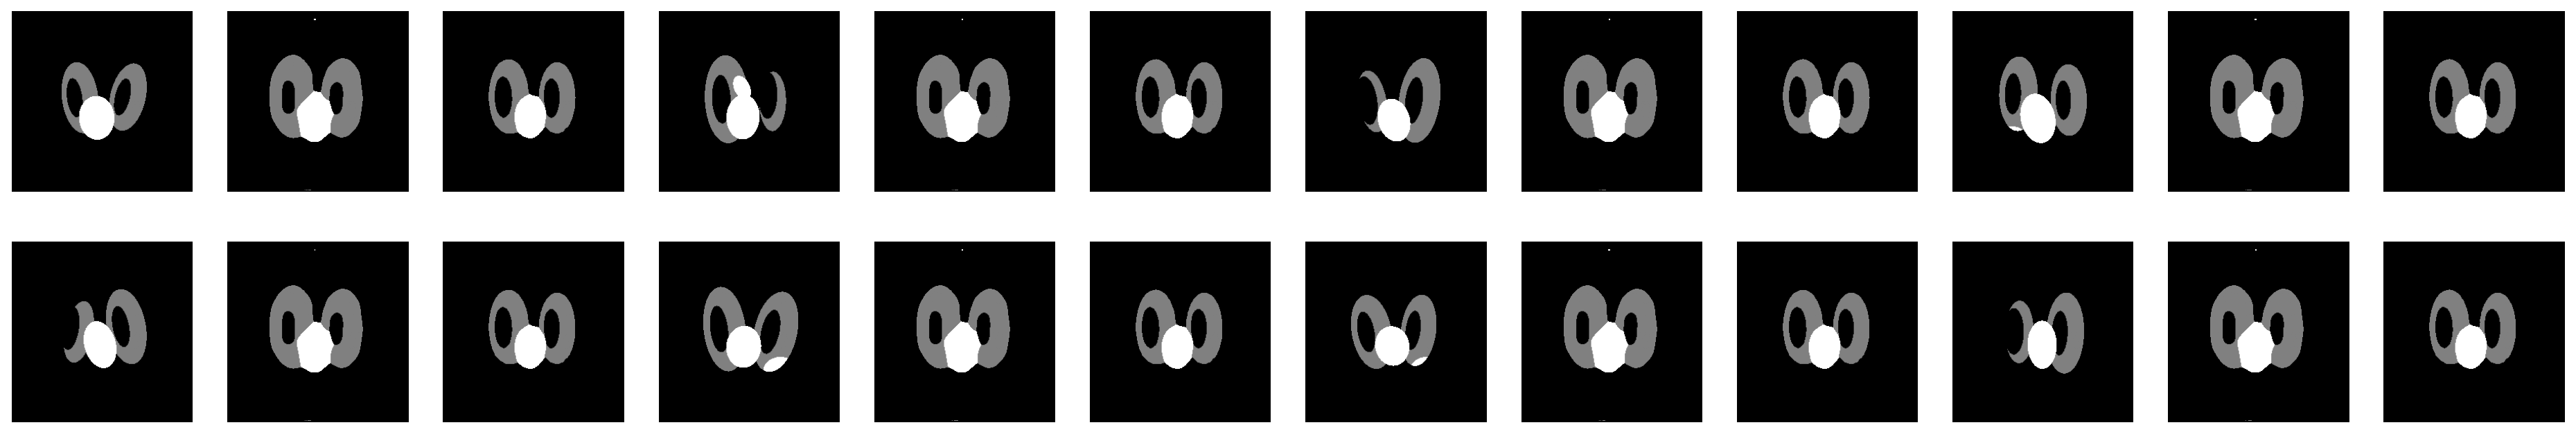
\includegraphics[width=0.96\linewidth]{../results/fcunet_lung2k_2/pulmonary_compare_1/test_comparison.png}
    \caption{Pulmonary synthetic test examples. Each triplet shows ground truth, DCT prediction, and FCUNet prediction.}
    \label{fig:pulmonary-compare}
\end{figure}

The data-scaling and efficiency summaries are also visualized in Figure~\ref{fig:pulmonary-summary}.

\begin{figure}[htbp]
    \centering
    \begin{subfigure}{0.48\linewidth}
        \centering
        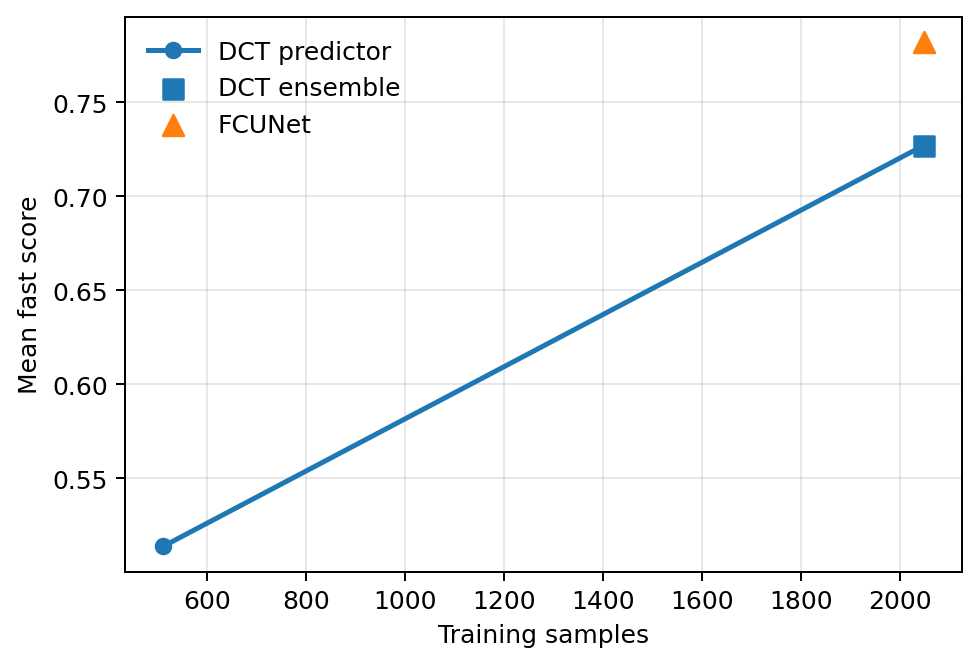
\includegraphics[width=\linewidth]{../results/pulmonary_summary_1/pulmonary_score_scaling.png}
    \end{subfigure}
    \hfill
    \begin{subfigure}{0.48\linewidth}
        \centering
        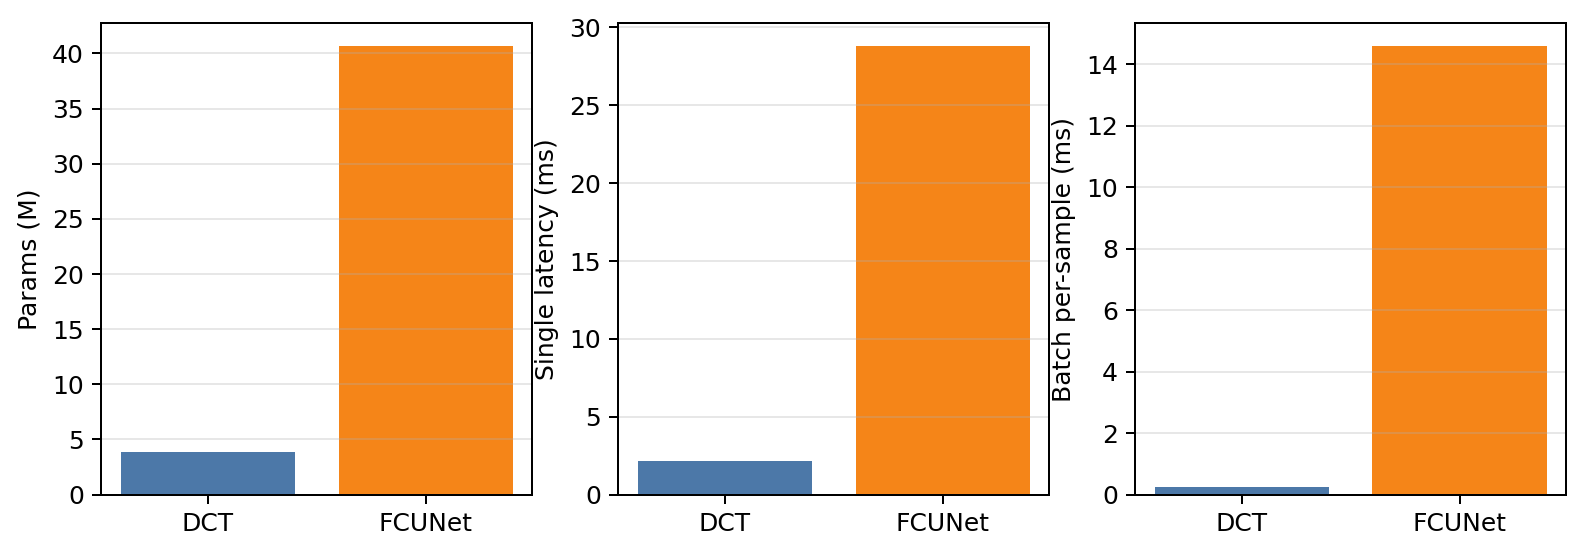
\includegraphics[width=\linewidth]{../results/pulmonary_summary_1/pulmonary_efficiency.png}
    \end{subfigure}
    \caption{Pulmonary DCT data scaling and DCT-vs-FCUNet efficiency comparison.}
    \label{fig:pulmonary-summary}
\end{figure}

\begin{figure}[htbp]
    \centering
    \begin{subfigure}{0.48\linewidth}
        \centering
        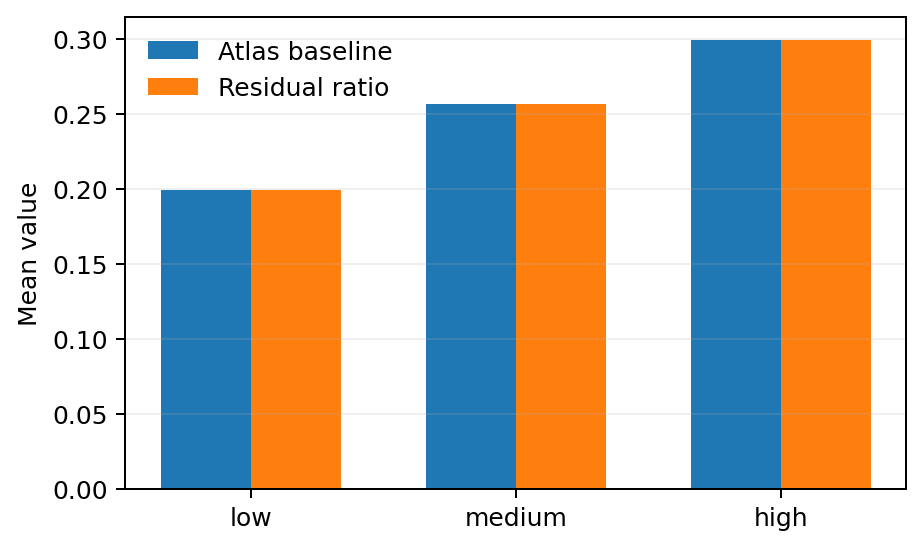
\includegraphics[width=\linewidth]{../results/lung_variability_analysis_2/summary_bars.png}
    \end{subfigure}
    \hfill
    \begin{subfigure}{0.48\linewidth}
        \centering
        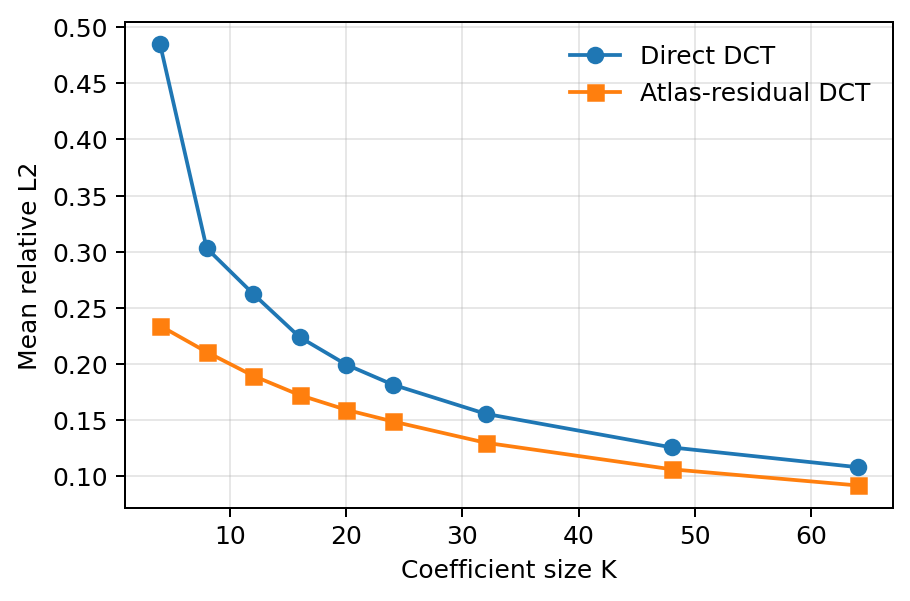
\includegraphics[width=\linewidth]{../results/pulmonary_complexity_2/dct_compressibility.png}
    \end{subfigure}
    \caption{Pulmonary complexity analysis. Left: atlas baseline strength under controllable low/medium/high generator settings. Right: direct DCT versus atlas-residual DCT compressibility on the `lung2k` test split.}
    \label{fig:pulmonary-complexity}
\end{figure}

\begin{figure}[htbp]
    \centering
    \begin{subfigure}{0.48\linewidth}
        \centering
        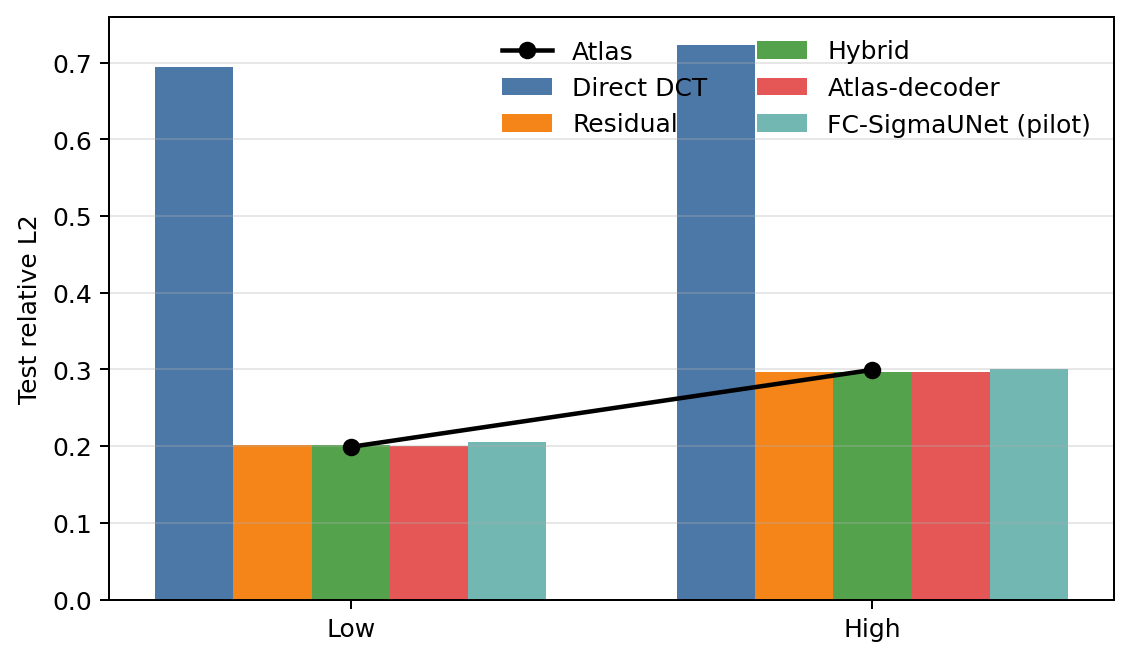
\includegraphics[width=\linewidth]{../results/pulmonary_complexity_models_3/complexity_bar.png}
    \end{subfigure}
    \hfill
    \begin{subfigure}{0.48\linewidth}
        \centering
        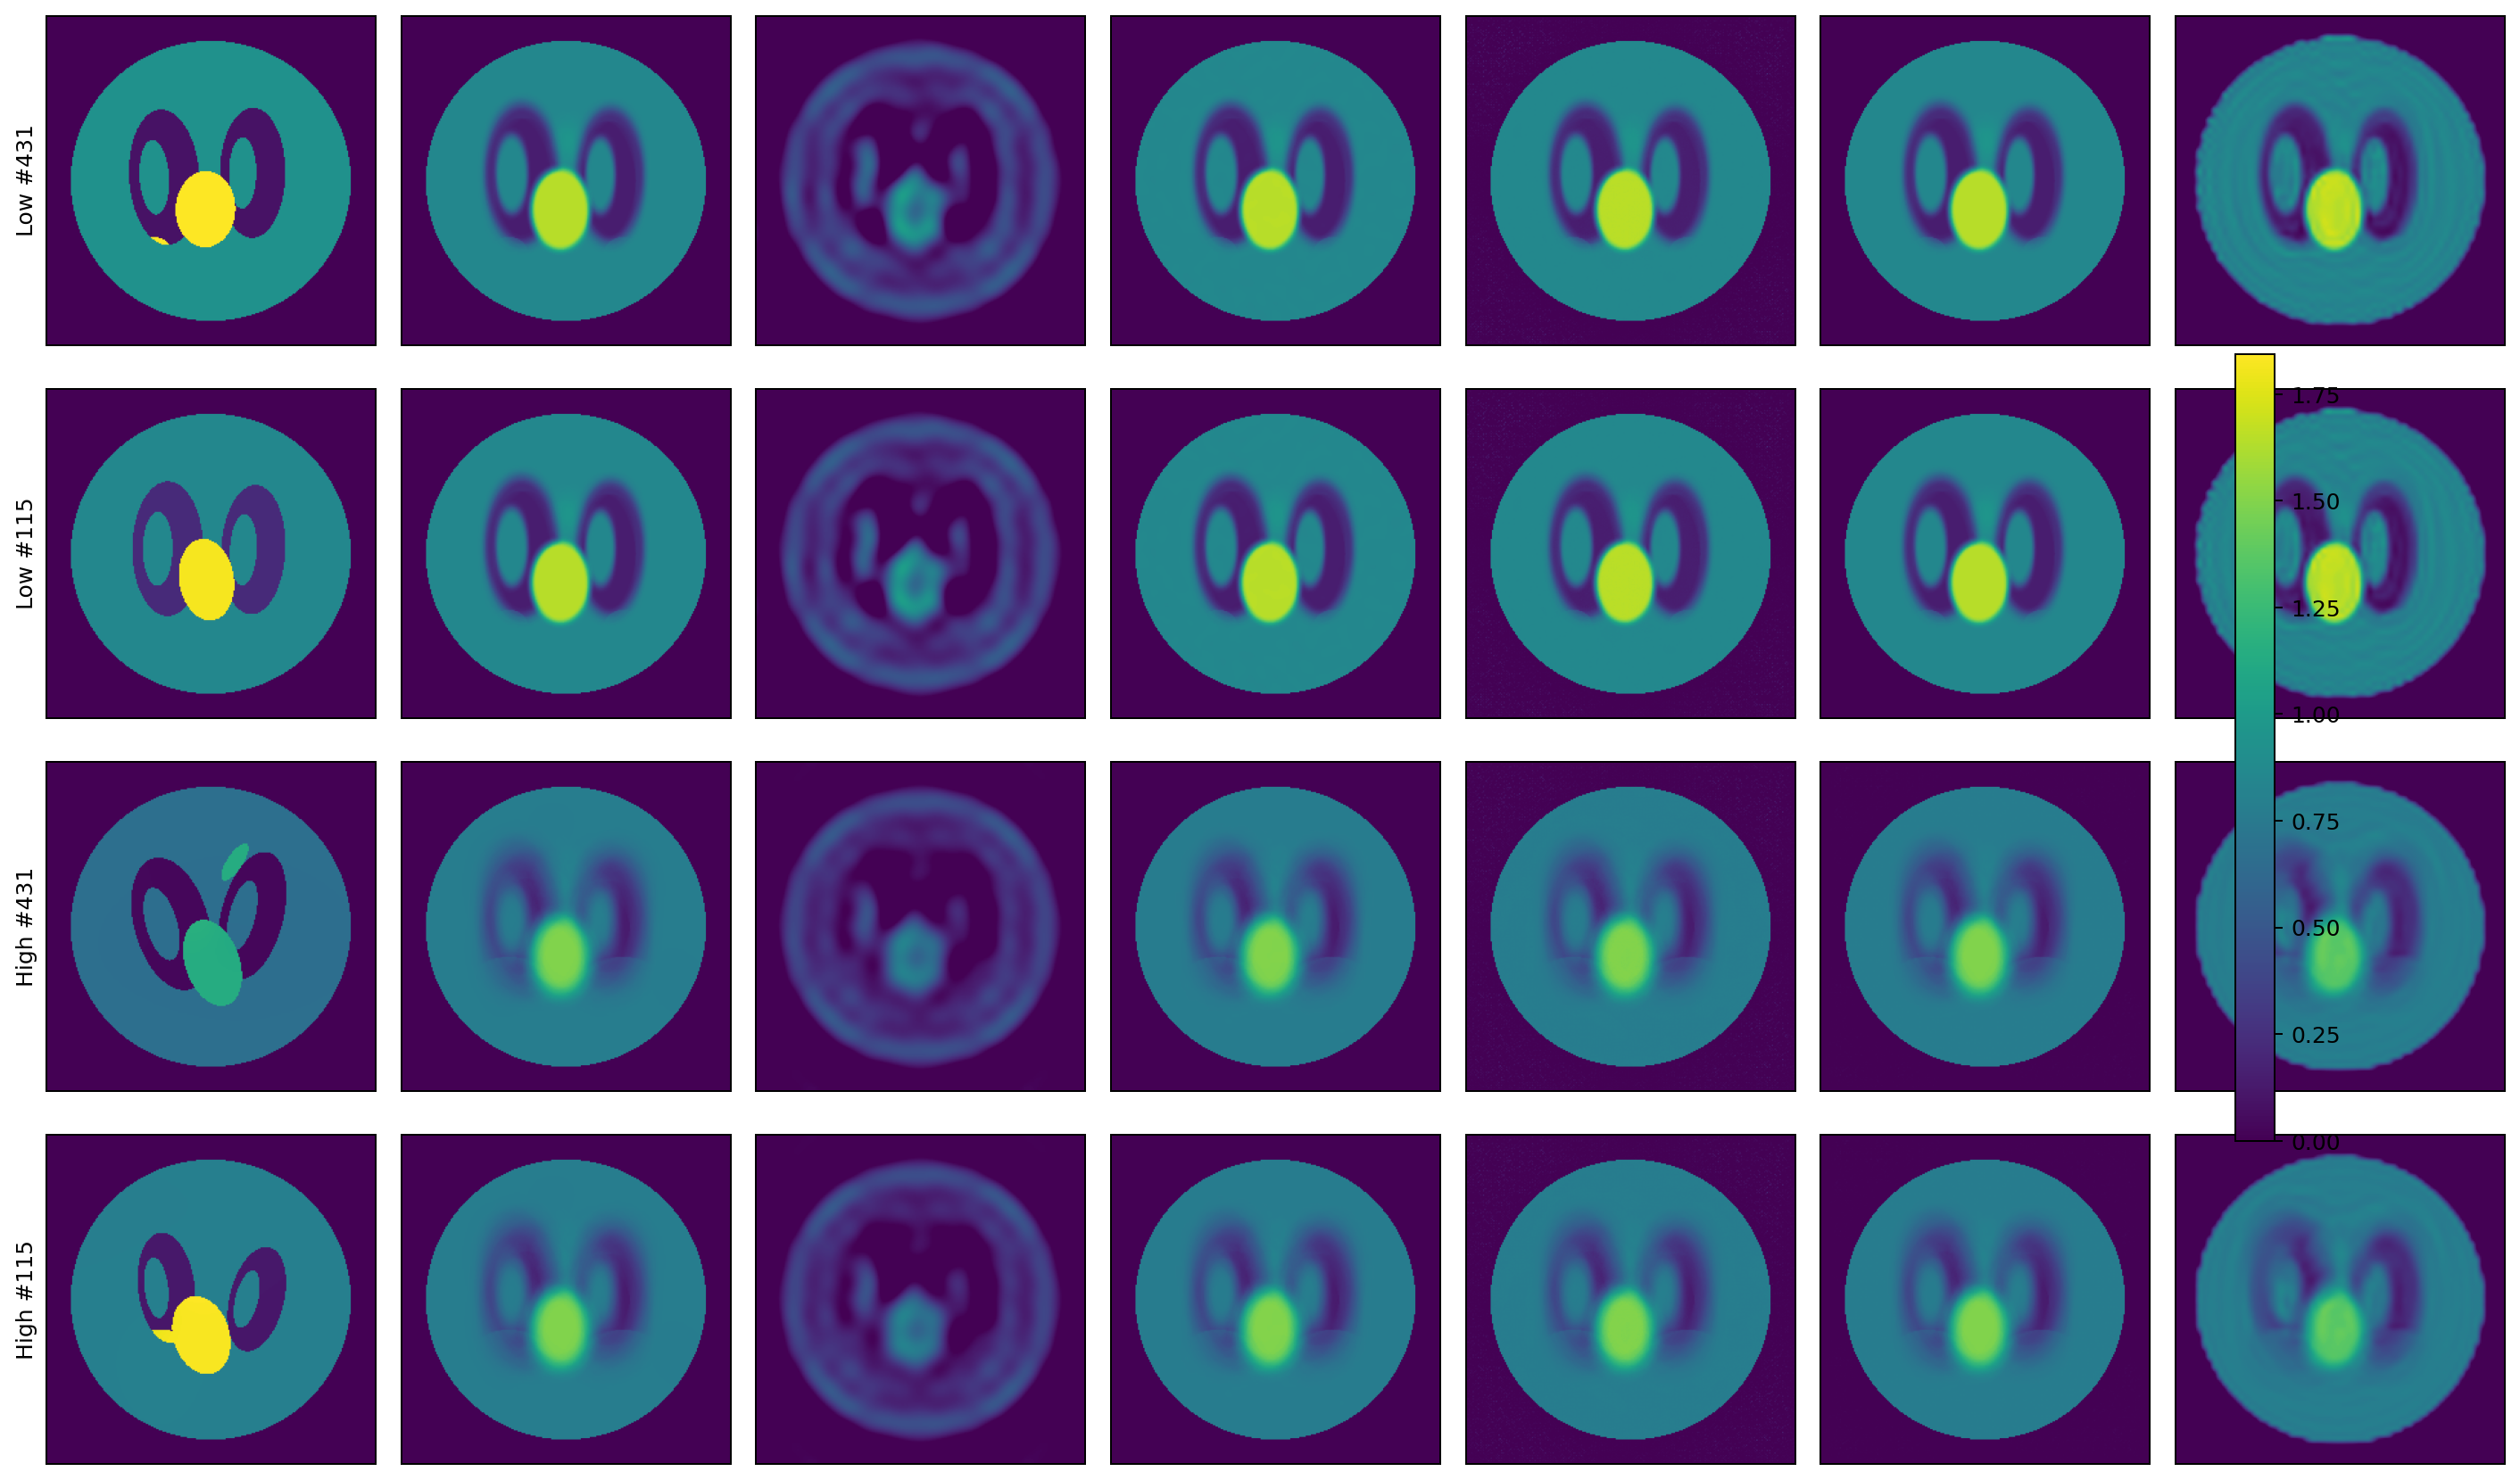
\includegraphics[width=\linewidth]{../results/pulmonary_complexity_visual_3/comparison.png}
    \end{subfigure}
    \caption{Matched low/high-complexity pulmonary conductivity comparison. Left: test relative-$L_2$ of direct DCT, atlas-residual DCT, hybrid DCT, atlas-decoder, and FC-SigmaUNet pilot against the atlas baseline. Right: qualitative examples showing GT, atlas, and the five model predictions under low and high complexity.}
    \label{fig:pulmonary-complexity-models}
\end{figure}

\section{Discussion}
The experiments show that once image-side regularization becomes strong enough, the dominant difficulty shifts to representation predictability from measurements. This explains why both continuous and discrete latent autoencoders can produce good reconstruction manifolds while still underperforming in end-to-end inversion.

The DCT results sharpen this conclusion. The main benefit does not come from raw model capacity, but from choosing a representation whose complexity matches the information content of EIT boundary measurements. Compared with learned latent spaces, the DCT basis is globally coupled, explicitly low-frequency, analytically decodable, and much easier to regress from measurements. These properties explain why it succeeds on the benchmark task even though more flexible latent methods do not.

At the same time, the pulmonary experiments reveal an important limitation: the representation family that is strongest on the benchmark phantom task is not automatically strongest on a more structured pulmonary synthetic task. FCUNet's richer spatial decoder currently yields better pulmonary reconstruction accuracy, suggesting that the pulmonary regime still benefits from more expressive image-space modeling. However, the DCT route remains highly attractive from an efficiency standpoint and improves substantially as data scale increases.

Our later pulmonary conductivity-regression experiments sharpen this point further. Once the global thorax shape is made explicit through a train-mean atlas, the remaining task becomes recovering small local deviations rather than reconstructing the whole anatomy from scratch. The matched low/high-complexity experiments confirm that direct DCT regression is structurally unstable in this regime, while atlas-residual, coarse-to-fine DCT, and atlas-decoder models recover the correct operating point and remain close to the atlas baseline. A short-run FC-SigmaUNet pilot baseline also stays in essentially the same range despite using a much heavier decoder. Residual-region evaluation further shows that these atlas-aware models remain essentially identical to the atlas baseline even on pixels with large atlas deviations, and the focus-loss ablation shows that simply reweighting those pixels is not enough to fix the problem. Because neither the learned atlas-decoder nor the heavier image-space baseline materially improve over the fixed-basis atlas-aware models, the evidence now points to measurement-to-residual inference as the bottleneck rather than decoder expressivity. This suggests that future pulmonary models should explicitly separate stable global anatomy from measurement-driven local perturbations, instead of treating the entire conductivity image as uniformly variable.

These observations suggest that the DCT predictor should be framed not only as an accuracy-driven method, but also as an efficiency-oriented pulmonary EIT method. In particular, its low parameter count and latency make it appealing for real-time systems, embedded deployment, and fast clinical monitoring settings where computational simplicity matters. From an ICIC perspective, the contribution is therefore broader than proposing another network: it combines fast simulation, accelerated evaluation, controllable pulmonary data complexity, and representation-aware reconstruction analysis in a single reproducible framework.

\section{Limitations and Future Work}
The current study still has four important limitations. First, although the proposed DCT method is strongest on the benchmark phantom task, it does not yet surpass FCUNet on the pulmonary synthetic task. This means the pulmonary claim should be framed as an efficiency-oriented contribution rather than as the best absolute reconstructor. Second, the pulmonary continuous-regression setting exposes a strong mean-atlas baseline, so future studies must report it explicitly and must demonstrate gains on local deviation recovery rather than only on global anatomy. Third, the current atlas-aware variants stabilize pulmonary behavior but still do not close the gap to the oracle atlas-residual DCT compressibility bound, residual-region metrics remain effectively tied to the atlas baseline, and even a learned atlas-decoder fails to materially improve over the fixed-basis atlas-aware models; this means the measurement-to-residual mapping remains under-optimized. Fourth, the real thoracic \texttt{.get} data available in the repository follow a 16-electrode, 208-channel regime, while the current KTC-style pipelines assume 32 electrodes and 2356 channels. A fully aligned pulmonary Sim2Real study therefore requires either a dedicated 16-electrode simulation pipeline or a matched external dataset.

The most promising next steps are therefore: (i) extending pulmonary experiments to larger synthetic datasets and multiple complexity levels, because the DCT route already shows both positive data-scaling and a strong sensitivity to atlas dominance; (ii) strengthening residual-focused objectives or local refinement modules so that atlas-aware DCT can improve beyond the atlas baseline instead of merely matching it; (iii) designing a 16-electrode training pipeline matched to the parsed real thoracic data; and (iv) broadening the baseline set so that the DCT method is compared against a larger family of pulmonary EIT networks rather than FCUNet alone.

\section{Conclusion}
This work provides a reproducible comparative study of representation choices for EIT reconstruction. The current evidence shows that:
\begin{itemize}[leftmargin=1.5em]
    \item FCUNet is a strong benchmark baseline.
    \item Pixel-wise discrete architectures are poorly matched to low-frequency conductivity structure.
    \item Continuous and discrete latent autoencoders improve image regularity but do not solve the inverse mapping bottleneck by themselves.
    \item A fixed low-frequency DCT parameterization achieves the best current benchmark result in the repository through a lightweight ensemble.
    \item On pulmonary synthetic data, FCUNet is currently the stronger reconstruction baseline, whereas the proposed DCT route offers a substantially better efficiency profile and clear positive data-scaling behavior.
    \item Pulmonary continuous-conductivity reconstruction is strongly atlas-dominated, so future progress depends on recovering local deviations around stable anatomy rather than on global image generation alone.
    \item Matched low/high-complexity pulmonary experiments show that atlas-aware DCT variants are necessary to stay aligned with the pulmonary data regime, while direct full-image DCT regression is structurally unstable, focus-loss reweighting has negligible effect, and a heavier FC-SigmaUNet pilot still does not escape the atlas-dominated operating point.
\end{itemize}

The next stage should therefore proceed in two parallel directions: stronger pulmonary baselines for absolute reconstruction quality, and further optimization of low-frequency fixed-basis predictors for efficient pulmonary EIT deployment.

\bibliographystyle{plain}
\bibliography{references}

\end{document}
